\documentclass{article}
\usepackage[margin=1.2in]{geometry}
\usepackage{datetime}
\usepackage{hyperref}      %for \url macro
\usepackage{microtype}     %attempt to fix issue with justification protrusion (in references)
\usepackage{amssymb}       % for formatting less/greater than symbols
\usepackage{amsmath}
\usepackage{enumitem}      %for changing spacing in bulleted lists
\usepackage{subfigure}        %for subfigures


\renewcommand{\arraystretch}{1.25}

\usepackage[gobble=auto, runall=true]{pythontex}
\usepackage{float} %for forcing position of images

\usepackage{graphicx}
\graphicspath{ {../images/} }
\usepackage[export]{adjustbox}
\usepackage[justification=centering]{caption}

\usepackage{listings}   %for typesetting code
\usepackage{color}
\definecolor{codegreen}{rgb}{0,0.6,0}
\definecolor{codegray}{rgb}{0.5,0.5,0.5}
\definecolor{codepurple}{rgb}{0.58,0,0.82}
\definecolor{backcolour}{rgb}{0.95,0.95,0.92}
\lstdefinestyle{mystyle}{
    backgroundcolor=\color{backcolour},
    commentstyle=\color{codegreen},
    keywordstyle=\color{codepurple},
    numberstyle=\tiny\color{codegray},
    stringstyle=\color{codepurple},
    basicstyle=\footnotesize,
    breakatwhitespace=false,
    breaklines=true,
    captionpos=b,
    keepspaces=true,
    %numbers=left,
    numbersep=5pt,
    showspaces=false,
    showstringspaces=false,
    showtabs=false,
    tabsize=2
}
\lstset{style=mystyle}

\frenchspacing                   %removes extra spacing after a period at the end of a sentence.
\newdateformat{daymonthyear}{\THEDAY\ \monthname\ \THEYEAR}

\title{CSC411 Machine Learning \\ Project 4: Reinforcement Learning}
\author{ Ariel Kelman \\ Student No: 1000561368
         \\ \\
         Gideon Blinick \\ Student No: 999763000 }
\daymonthyear



\begin{document}
   \maketitle{}


   \section{Introduction}
   \subsection{Results \& Report Reproducibility}
   All results and plots can be generated using the code in \texttt{tictactoe.py}.
   All code is python 3, run with Anaconda 3.6.3.
   Running the code will save all generated images in the \texttt{resources} folder,
   where they are used by \LaTeX. Note that some of the sections require the code for
   other sections (in the same file) to be run first.
   To reproduce the report, simply run it through \LaTeX. This will pull the most recently
   generated figures from the \texttt{resources} folder.

   \subsection{Tic Tac Toe Environment}
   The \texttt{Environment} class provides the functionality required to play a game of tic tac
   toe, including against an opponent who plays a random legal move. The game is represented by the
   \texttt{grid} attribute, which is a \texttt{numpy} array representing the $9$ positions. Each position
   can have a $0, 1$ or $2$, representing an empty position, or one filled by player 1 ($X$) or 2 ($O$)
   respectively. The \texttt{turn} attribute can have a value of $1$ or $2$, and represents which player
   has the next move. The \texttt{done} attribute is a boolean that indicates whether a game has been
   completed (either with a win, or when the board is full).

   The \texttt{step()} and \texttt{render()} methods allow a tic tac toe game to be played and displayed
   with text output. Using these methods, a game was played, resulting in the following text output:
   \begin{lstlisting}[language=Python]

      ...
      .x.
      ...
      ====
      o..
      .x.
      ...
      ====
      o.x
      .x.
      ...
      ====
      o.x
      ox.
      ...
      ====
      o.x
      ox.
      x..
      ====
   \end{lstlisting}


   \section{Policy}
   The \texttt{Policy} class implements a neural network that learns to play tic tac toe. The provided
   starter code was modified to be a one-hidden layer neural network; the final code is shown in the
   code block below.
   \begin{lstlisting}[language=Python, label={PolicyClass}]

      class Policy(nn.Module):
         """
         The Tic-Tac-Toe Policy
         """
         def __init__(self, input_size=27, hidden_size=64, output_size=9):
              super().__init__()
              self.Linear1 = nn.Linear(input_size, hidden_size)
              self.Linear2 = nn.Linear(hidden_size, output_size)

         def forward(self, x):
              h = F.relu( self.Linear1(x) )
              out = F.softmax( self.Linear2(h) )
              return out
   \end{lstlisting}

   In choosing an action, the state is represented as a 27-dimensional vector, using a one-hot encoding
   type scheme. The first nine elements are $1$ if the corresponding location (moving horizontally, and then
   from top to bottom), and $0$ otherwise. Similarly, the next $9$ elements are $1$ if an $X$ (representing
   player 1) is in the corresponding location; while the last nine elements provide the same functionality
   for $O$ (player 2).

   The policy outputs a nine-dimensional vector, which is a probability distribution that is sampled to choose
   the move for the policy. Thus the policy is stochastic - the \texttt{select\_action()} function samples this
   distribution to choose a move.


   \section{Policy Gradient}
   The \texttt{compute\_returns()} function computes the returns based on the reward at the end of a game.
   The following code block shows how the returns are calculated.
   \begin{lstlisting}[language=Python, label={returns}]

      def compute_returns(rewards, gamma=1.0):
         """
         Compute returns for each time step, given the rewards
         """
         k = len(rewards)
         rewards = np.array(rewards)
         gammas = np.array( [gamma**(i) for i in range(k) ] )
         G = [ sum( rewards[i:]*gammas[:k-i] ) for i in range(k) ]
         return G
   \end{lstlisting}

   The weights are updated on the conclusion of a game, though this means that the policy does not improve
   during a game (this is a minor cost considering how short the games are). For updates to the policy to have
   any meaning in the middle of the game, there would need to be rewards for intermediate states. This would
   require having a metric that evaluates a tic tac toe position. While this could be done in tic tac toe,
   it would be quite difficult in more complicated games, where it is not obvious how a position should be
   rewarded. Having rewards only at the end still improves the policy choices earlier in the game (if an early
   position leads to a win, that position will be wieghted more positively when propogating backwards).
   Thus updating the weights at the end of an episode provides a simple way to provide feedback and improve the
   policy.

   \section{Rewards}
   When originally setting the rewards (in the \texttt{get\_reward()} function), they were set as shown in
   table \ref{table:part4}.
      \begin{table}[h]
         \centering
         \renewcommand{\arraystretch}{1.5}

         \begin{tabular}{ p{8em}|l }
            \hline
            status     &     reward      \\
            \hline \hline
            VALID\_MOVE       &  1       \\
            INVALID\_MOVE     &  -10     \\
            WIN               &  15      \\
            TIE               &  3       \\
            LOSE              &  -1      \\
            \hline
         \end{tabular}

         \caption{ Original rewards (the \texttt{DONE} status was not give a reward). }
         \label{table:part4}
      \end{table}
   The logic behind these rewards was to follow an intuitive feeling for how much the above results
   are actually desired. This is somewhat arbitrary, but does represent a reasonable starting point.
   Thus a valid move should get a small positive reward, while an invalid one should
   be heavily penalized. A win is highly rewarded, a tie gets some reward for preventing a loss, while a
   loss is penalized (it would have been reasonable to start with a more negative penalty here too).
   The \texttt{DONE} status was not given a reward; that scenario is taken care of by the \texttt{TIE} status.

   However, while debugging during training, the rewards were set to much simpler values, and - since
   after the issues were resolved the win rate was quite high - the changed rewards were kept. These rewards
   were simply $+1$ for a win, and $-1$ for an invalid move.
   A side-effect of this scheme is that the average return is equivalent to the win rate.

   The final \texttt{get\_reward()} function is shown in the following code block.
      \begin{lstlisting}[language=Python, label={reward}]

         def get_reward(status):
            """Returns a numeric given an environment status."""
            return {
                     Environment.STATUS_VALID_MOVE  : 0,
                     Environment.STATUS_INVALID_MOVE: -1,
                     Environment.STATUS_WIN         : 1,
                     Environment.STATUS_TIE         : 0,
                     Environment.STATUS_LOSE        : 0
            }[status]
      \end{lstlisting}


   \section{Training}
   \subsection{Learning Curve}
   Figure \ref{fig:5a} shows a learning curve, showing the average returns of the 1000 previous episodes. Note
   that the policy is modified throughout these episodes. The policy has one hidden layer with 64 hidden neurons
   (this is the default value that will be experimented with in the next subsection), a RELU activation, as well
   as a softmax layer on the output (to convert the output to a probability distribution). A gamma of $0.99$ was used
   to discount the rewards. Using a gamma of $1$ lowered the average returns and win rate by over 10\% (plots showing
   these results can be found in the \texttt{resources} folder).
      \begin{figure}[h] \centering
          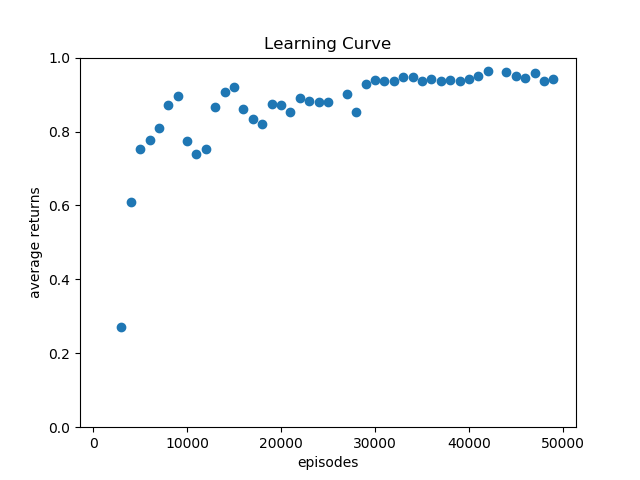
\includegraphics[width=4in]{resources/part5a_scaled}
          \caption{ Learning curve showing the average return as a function of the number of episodes
                  that have been played. Only points in the interval $[0,1]$ are shown (this gave the best scale),
                  though there are points with lower average returns (a plot with all points is saved
                  as \texttt{part5a\_allPoints} in the \texttt{resources} folder). }
          \label{fig:5a}
       \end{figure}

   \subsection{Hidden Units}
   The value of 64 hidden neurons gave excellent results as shown in figure \ref{fig:5a}, but changes to this value
   were explored to show how results changed as this number was varied.
      \begin{table}[h]
         \centering
         \renewcommand{\arraystretch}{1.5}

         \begin{tabular}{ p{7em}|l|l|l }
            \hline
            number of hidden units     &     win rate \% & avg returns & invalid moves \%   \\
            \hline \hline
            2     &  61.3   & -1.4   &  33    \\
            9     &  91.4   & 0.88   &  0.5   \\
            27    &  93.6   & 0.94   &  0.1   \\
            64    &  93.9   & 0.94   &  0     \\
            100   &  93.9   & 0.94   &  0     \\
            \hline
         \end{tabular}

         \caption{ Win rate after 50000 episodes varying with the number of hidden units in the policy. The win rate
                  shown was found by playing the policy against a random opponent for 1000 games. }
         \label{table:part5b}
      \end{table}
   Table \ref{table:part5b} shows several metrics for evaluation the policy after 50000 episodes. 2 hidden neurons
   clearly do not have enough capacity to form a good policy, while 9 preforms pretty well (much higher than the
   60\% baseline win rate for a random player with the first move), and 27 is already almost indistinguishable from 100.

   \subsection{Invalid Moves}
   Figure \ref{fig:5c} shows the fraction of all moves played by the learned policy that were invalid. As above, each
   point is the average over the previous 1000 episodes. Looking at the graph, invalid moves have pretty much
   completely stopped before the 10000th episode (less than 1 \%), though there are still statistical fluctuations
   to much higher rates of invalid moves.
      \begin{figure}[h] \centering
          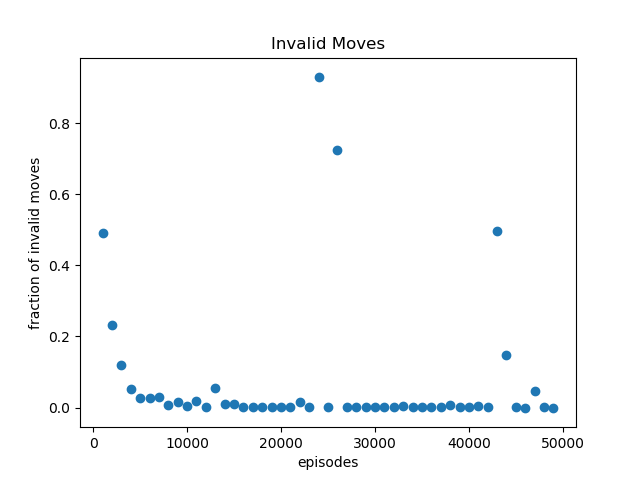
\includegraphics[width=4in]{resources/part5c}
          \caption{ Fraction of invalid moves varying with the number of episodes that have been played as
                  part of training. }
          \label{fig:5c}
       \end{figure}

   \subsection{Win-Lose-Tie Ratios}
   Playing the trained policy against a randomized opponent for 100 games, the policy (which went first as $X$)
   won 95, lost 3, and tied 2. This is an excellent policy; note that the losing and tying rates are quite similar,
   which is to be expected, as they are both given no reward.

   Figure \ref{fig:5d} shows 5 sample games, each of which was won by the policy in 3 turns (these games are
   five new games, not included in the 100 above, though presumably many of those games were quite similar).
      \begin{figure}[h] \centering
          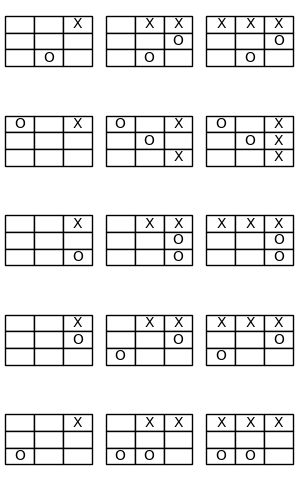
\includegraphics[width=4in]{resources/part5d}
          \caption{ A sample of 5 games played by the trained policy against a random opponent. The games
                  move from left to right. The image was generated by the \texttt{display\_games()} function. }
          \label{fig:5d}
       \end{figure}
   The policy seems to have learned that a corner is the best move, but it does not seem to have developed more
   advanced strategies than that (such as the double-trap). Sampling another 10 games (saved as \texttt{part5d\_more}
   in the \texttt{resources} folder) actually shows some bad strategy, such as not closing off an opportunity for
   $O$ to win; thus showing a weakness of the rewards that were used. Also noteworthy is that the policy seems to
   have learned that the middle square is not a good move - in only 2/15 of the sampled games is that moved played; in
   the rest, the policy wins along an edge.

   \section{Win Rate over Episodes}
   Figure \ref{fig:6} shows, using weights stored throughout training (every 1000 episodes), how the win, lose,
   and tie rates changed as training progressed. Each set of weights was loaded, and then played 1000 games against
   a random opponent to determine these numbers.
      \begin{figure}[h] \centering
          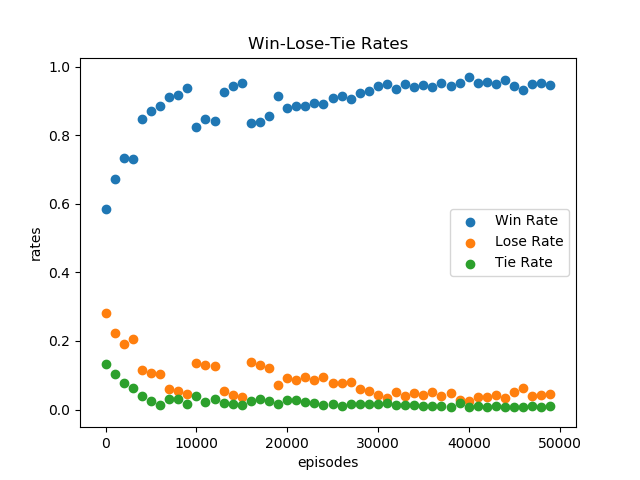
\includegraphics[width=4in]{resources/part6}
          \caption{ Win-Lose-Tie Ratios }
          \label{fig:6}
       \end{figure}
   Several interesting results can be observed: as expected, the win rate increases steadily while both the losing
   and tying rates decrease. There are greater statistical fluctuations towards the beginning of training, where
   wins are ``replaced'' by unexpected losses. Though the losing rate is generally higher than the tying rate (despite
   the similar rewards for both scenarios), this is likely due to tying being a more unlikely outcome in tic tac toe (at
   least where one of the players is random while the other is highly trained; it's well known that for optimal play
   games always end in a tie).

   \section{First Moves}
   \section{Limitations}


\end{document}
